\documentclass{standalone}
\usepackage{tikz}
\begin{document}
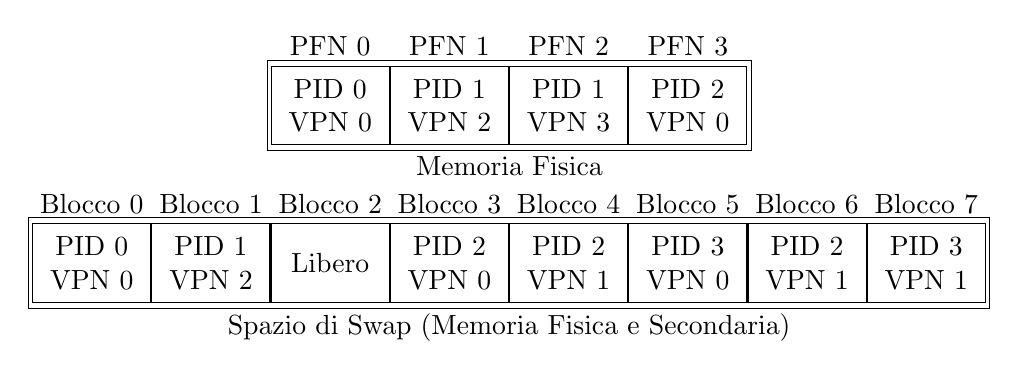
\begin{tikzpicture}
    \draw

    %% **
    % node[draw, rectangle, minimum length=1.5cm, minimum height=1cm, fill=white, anchor=180](e1){}

    (-0.05,-1)node[draw, rectangle, minimum height=1.15cm, minimum width=12.2cm, anchor=180, label={[label distance=-1.7cm]:Spazio di Swap (Memoria Fisica e Secondaria)}]{}
    (0,-1)node[draw, rectangle, minimum width=1.5cm, minimum height=1cm, fill=white, align=center, anchor=180, label={Blocco 0}](e0){PID 0\\VPN 0}
    (e0.0)node[draw, rectangle, minimum width=1.5cm, minimum height=1cm, fill=white, align=center, anchor=180, label={Blocco 1}](e1){PID 1\\VPN 2}
    (e1.0)node[draw, rectangle, minimum width=1.5cm, minimum height=1cm, fill=white, align=center, anchor=180, label={Blocco 2}](e2){Libero}
    (e2.0)node[draw, rectangle, minimum width=1.5cm, minimum height=1cm, fill=white, align=center, anchor=180, label={Blocco 3}](e3){PID 2\\VPN 0}
    (e3.0)node[draw, rectangle, minimum width=1.5cm, minimum height=1cm, fill=white, align=center, anchor=180, label={Blocco 4}](e4){PID 2\\VPN 1}
    (e4.0)node[draw, rectangle, minimum width=1.5cm, minimum height=1cm, fill=white, align=center, anchor=180, label={Blocco 5}](e5){PID 3\\VPN 0}
    (e5.0)node[draw, rectangle, minimum width=1.5cm, minimum height=1cm, fill=white, align=center, anchor=180, label={Blocco 6}](e6){PID 2\\VPN 1}
    (e6.0)node[draw, rectangle, minimum width=1.5cm, minimum height=1cm, fill=white, align=center, anchor=180, label={Blocco 7}](e7){PID 3\\VPN 1}

    
    (e1.0)++(-0.05,2)node[draw, rectangle, minimum height=1.15cm, minimum width=6.15cm, anchor=180, label={[label distance=-1.6cm]:Memoria Fisica}]{}
    (e1.0)++(0,2)node[draw, rectangle, minimum width=1.5cm, minimum height=1cm, fill=white, align=center, anchor=180, label={PFN 0}](e1){PID 0\\VPN 0}
    (e1.0)node[draw, rectangle, minimum width=1.5cm, minimum height=1cm, fill=white, align=center, anchor=180, label={PFN 1}](e1){PID 1\\VPN 2}
    (e1.0)node[draw, rectangle, minimum width=1.5cm, minimum height=1cm, fill=white, align=center, anchor=180, label={PFN 2}](e1){PID 1\\VPN 3}
    (e1.0)node[draw, rectangle, minimum width=1.5cm, minimum height=1cm, fill=white, align=center, anchor=180, label={PFN 3}](e1){PID 2\\VPN 0}



    ;
\end{tikzpicture}
\end{document}